\documentclass[tikz, border=3mm]{standalone}
\usepackage{tikz}
\usepackage{amsmath} % For \frac, \pi
\usetikzlibrary{arrows.meta, decorations.markings, angles, quotes, calc}

\begin{document}
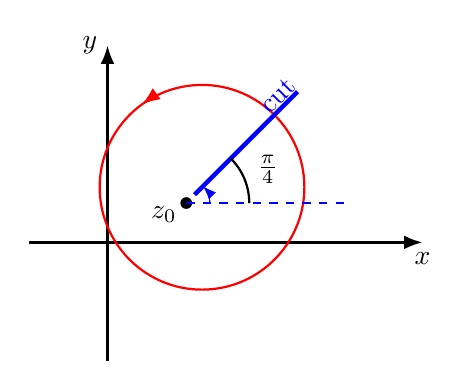
\begin{tikzpicture}[
    >=Latex, % Set default arrow tip style
    dot/.style={fill=black, circle, inner sep=1.5pt} % Style for points
]

% Axes
\draw[->, thick] (-1, 0) -- (4, 0) node[below] {$x$};
\draw[->, thick] (0, -1.5) -- (0, 2.5) node[left] {$y$};

% Define z0 coordinate and circle parameters
\coordinate (z0) at (1, 0.5);
\coordinate (center) at (1.2, 0.7); % Center slightly offset from z0
\def\radius{1.3} % Circle radius

% Draw the red closed curve (circle)
\draw[red, thick,
    postaction={decorate, decoration={markings, mark=at position 0.35 with {\arrow{>}}}} % Counter-clockwise arrow near top-left
] (center) circle (\radius);

% Draw the point z0 and label it
\node[dot, label={[below left]$z_0$}] at (z0) {};

% Define cut angle and points
\def\cutangle{45} % Angle of the cut line in degrees
\coordinate (cutstart) at ($(z0)+(\cutangle:0.15)$); % Start cut slightly away from z0
\coordinate (cutend) at ($(z0)+(\cutangle:2.0)$);   % End cut further out

% Draw the cut line
\draw[blue, ultra thick] (cutstart) -- (cutend);
\node[blue, above right, rotate=\cutangle, inner sep=1pt] at ($(z0)+(\cutangle:1.5)$) {cut};

% Draw dashed horizontal line segment from z0
\coordinate (z0horz) at ($(z0)+(2.0,0)$); % Short horizontal segment
\draw[dashed, blue] (z0) -- (z0horz);

% Draw angle pi/4
\pic [draw, thick, angle radius=0.8cm, "$\frac{\pi}{4}$", angle eccentricity=1.4] {angle = z0horz--z0--cutend};

% Draw small blue angle arc near z0
\pic [draw, blue, ->, angle radius=0.3cm] {angle = z0horz--z0--cutend};

% Draw thick red arc on circle near horizontal intersection
% Estimate intersection angle (approx -15 deg for these parameters)
\def\intersectangle{-15}
%\draw[red, ultra thick] (center) + ({\intersectangle}:\radius) arc ({\intersectangle}:{\intersectangle+10}:\radius);


\end{tikzpicture}
\end{document}